\documentclass[acmsmall,screen]{acmart}
\setcopyright{none}
\acmDOI{}
\acmISBN{}
\acmJournal{CSUR}
\settopmatter{printacmref=true}
\raggedbottom
\acmYear{2026}
\acmVolume{1}
\acmNumber{1}
\acmArticle{1}

\usepackage{amsmath}
\usepackage{booktabs}
\usepackage{tabularx}
\usepackage{array}
\usepackage{multirow}
\usepackage{tikz}
\usetikzlibrary{arrows.meta,positioning,shapes.geometric,fit}
\usepackage{enumitem}
\usepackage{microtype}

\newcolumntype{Y}{>{\raggedright\arraybackslash}X}
\newcolumntype{P}[1]{>{\raggedright\arraybackslash}p{#1}}

\title{Benchmarking Citation Fabrication Rates Across Large Language Models and Agentic Search Tools}
\author{Bayyapu Vamshidhar Reddy}
\affiliation{\institution{Indian Institute of Information Technology Allahabad}\city{Prayagraj}\country{India}}

\keywords{citation fabrication, citation hallucination, large language models, retrieval-augmented generation, agentic search, deep research agents, scientific integrity, reference verification, benchmarking}
\ccsdesc[500]{Computing methodologies~Natural language processing}
\ccsdesc[300]{Information systems~Digital libraries and archives}
\ccsdesc[200]{Information systems~Information retrieval}

\begin{document}
\begin{abstract}
Large language models (LLMs) and the agentic search and ``deep research'' tools built on top of them are increasingly used to locate, summarize, and cite scholarly and professional literature. A growing body of empirical work shows that these systems routinely generate citations to sources that do not exist, misattribute real sources, or link to URLs with no retrievable content --- a failure mode this paper terms citation fabrication. This review synthesizes benchmarking studies published between 2023 and 2026 across biomedicine, law, computer science, and general-purpose search to compare fabrication rates across base LLMs (e.g., GPT-3.5, GPT-4, Bard/Gemini), citation-augmented generation benchmarks (e.g., ALCE, FActScore), retrieval-augmented professional tools (e.g., commercial legal-research assistants), and autonomous ``deep research'' agents (e.g., OpenAI Deep Research, Gemini Deep Research, Perplexity Deep Research). Reported fabrication rates range from roughly 6\% to 91\% depending on system, domain, prompt, and verification method, with unaugmented chat models generally fabricating references most often, retrieval-augmented professional tools reducing but not eliminating the problem (17--33\%), and agentic deep-research systems presenting a distinct profile --- producing more citations per query while hallucinating source URLs at rates of roughly 3--18\%. The paper further reviews detection and mitigation approaches (self-verification, retrieval grounding, post-hoc reference checking) and documents the downstream contamination of the peer-reviewed scientific record itself. It closes by identifying methodological gaps --- inconsistent definitions of ``hallucination,'' a lack of standardized cross-system benchmarks, and the opacity of proprietary agentic pipelines --- and proposes directions for a more rigorous, comparable science of citation reliability.
\end{abstract}

\maketitle

\section{Introduction}\label{sec:introduction}
The rapid adoption of large language models (LLMs) as research assistants has created a new and consequential failure mode: the confident generation of bibliographic citations that are fluent, well-formatted, and entirely or partially false. Because a citation is a compact, independently verifiable claim --- a work either exists with the stated authors, venue, and year, or it does not --- citation fabrication has become one of the most tractable lenses through which to study the broader phenomenon of LLM ``hallucination'' \citep{agrawal2023,ji2023}.

The scale of the problem is no longer anecdotal. A large-scale audit of 111 million references across 2.5 million papers on arXiv, bioRxiv, SSRN, and PubMed Central found a sharp rise in non-existent citations coinciding with the widespread adoption of LLMs, with a conservative estimate of 146,932 hallucinated citations appearing in the 2025 literature alone \citep{zhao2026}. Fabricated citations have been documented inside peer-reviewed proceedings at flagship venues such as NeurIPS and USENIX Security \citep{russinovich2026b}, across hundreds of papers at ACL, NAACL, and EMNLP \citep{sakai2026}, and in award-winning submissions \citep{ansari2026}. Outside of academia, fabricated case citations generated by ChatGPT famously led to court sanctions in Mata v. Avianca and have since recurred in numerous other filings, prompting systematic study of legal-domain hallucination \citep{dahl2024,magesh2025}.

At the same time, the ecosystem of tools that people use to find citations has diversified well beyond a single chat window. Retrieval-augmented generation (RAG) pipelines, commercial ``AI research assistants'' built into legal and medical databases, and autonomous ``agentic search'' or ``deep research'' products (OpenAI Deep Research, Google Gemini Deep Research, Perplexity Deep Research, and comparable systems) now issue their own search queries, read multiple web pages, and synthesize long-form reports with inline citations \citep{du2025,rao2026}. Vendors have explicitly marketed retrieval grounding as a solution that renders citations ``hallucination-free'' \citep{magesh2025}, making an empirical, comparative assessment of that claim a matter of practical and scientific importance.

This paper reviews and synthesizes the available benchmarking evidence to answer three questions: (1) How prevalent is citation fabrication across different classes of systems --- bare LLMs, citation-oriented generation benchmarks, retrieval-augmented professional tools, and agentic deep-research systems? (2) What methods exist to detect and mitigate citation fabrication, and how effective are they? (3) What methodological and infrastructural gaps limit the field's ability to produce comparable, trustworthy benchmarks going forward? The paper is organized as follows. Section~\ref{sec:background} reviews related work on hallucination broadly and citation fabrication specifically. Section~\ref{sec:taxonomy} presents a comparative technical discussion of fabrication rates, organized by system class, including a summary table. Section~\ref{sec:mitigation} surveys current detection and mitigation approaches. Section~\ref{sec:challenges} discusses methodological challenges and limitations of the existing literature. Section~\ref{sec:gaps} identifies research gaps and future directions. Section~\ref{sec:conclusion} concludes.

\section{Review Methodology}\label{sec:methodology}
This review follows a structured evidence-synthesis workflow rather than treating the literature as a collection of independent paper summaries. The review scope covers empirical studies and benchmarks published from 2023 through September 2026 that evaluate citation existence, bibliographic correctness, citation support, or URL validity in LLM-based systems. The corpus spans four application settings: general-purpose chat models, citation-grounded generation, domain-specific retrieval-augmented systems, and autonomous deep-research agents.

The inclusion criteria were: (i) the study evaluates a named model, system, benchmark, or verification pipeline; (ii) citation or source reliability is measured explicitly or through a reproducible proxy; (iii) the study reports enough methodological detail to interpret its metric; and (iv) the publication is traceable to a scholarly venue, publisher, or persistent preprint record. Studies were excluded when they discussed hallucination only conceptually, reported no citation-related evidence, or could not be independently located. This process is important because the reported rates in the field are sensitive to prompt, domain, sample size, and the definition of failure.

The synthesis uses three analytical layers. First, \emph{existence} asks whether the cited work or URL corresponds to a real source. Second, \emph{attribute accuracy} asks whether authorship, title, venue, year, and identifiers are correct. Third, \emph{support accuracy} asks whether the cited source actually supports the claim for which it is presented. These layers prevent a real but irrelevant citation from being treated as equivalent to a completely fabricated work. The evidence map in Figure~\ref{fig:review-workflow} summarizes this review process.

\begin{figure*}[t]
\centering
\resizebox{0.96\textwidth}{!}{%
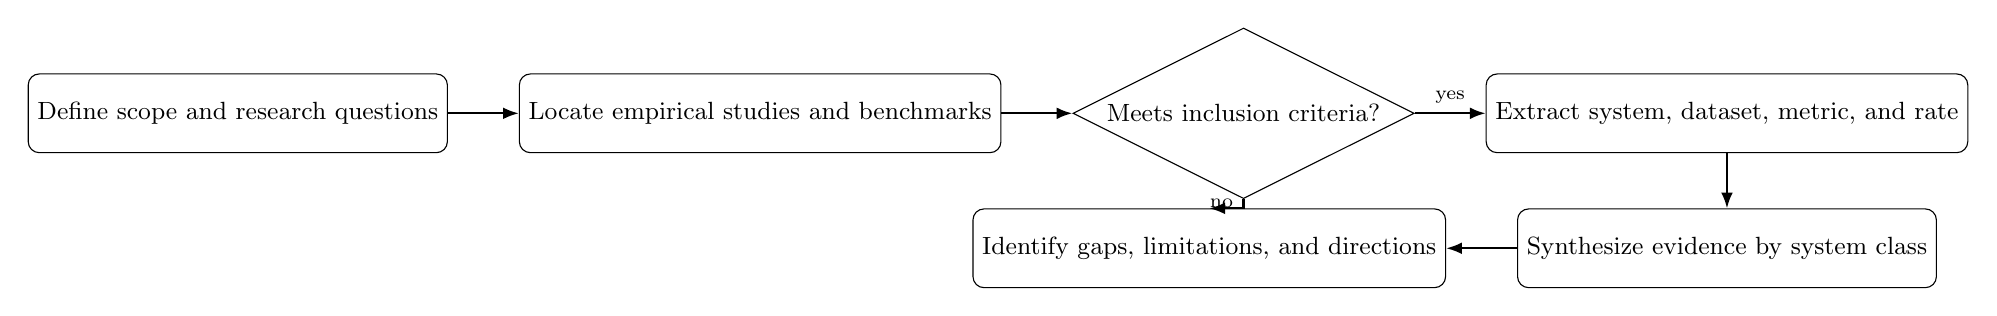
\begin{tikzpicture}[
  node distance=7mm and 9mm,
  box/.style={draw, rounded corners, align=center, minimum width=34mm, minimum height=10mm, font=\small},
  decision/.style={draw, diamond, aspect=2, align=center, inner sep=2pt, font=\small},
  arrow/.style={-{Latex[length=2mm]}, thick}
]
\node[box] (scope) {Define scope and research questions};
\node[box, right=of scope] (search) {Locate empirical studies and benchmarks};
\node[decision, right=of search] (screen) {Meets inclusion criteria?};
\node[box, right=of screen] (extract) {Extract system, dataset, metric, and rate};
\node[box, below=of extract] (synth) {Synthesize evidence by system class};
\node[box, left=of synth] (gaps) {Identify gaps, limitations, and directions};
\draw[arrow] (scope) -- (search);
\draw[arrow] (search) -- (screen);
\draw[arrow] (screen) -- node[above,font=\scriptsize]{yes} (extract);
\draw[arrow] (extract) -- (synth);
\draw[arrow] (synth) -- (gaps);
\draw[arrow] (screen.south) |- node[pos=.25,left,font=\scriptsize]{no} (gaps.north);
\end{tikzpicture}%
}
\caption{Structured workflow used to organize and synthesize the reviewed evidence.}
\Description{Flowchart showing the review process from scope definition through study search, inclusion screening, evidence extraction, synthesis, and research-gap identification.}
\label{fig:review-workflow}
\end{figure*}

\section{Background and Related Work}\label{sec:background}
\subsection{Hallucination as a general phenomenon}
``Hallucination'' in natural language generation refers to generated content that is fluent and plausible but unsupported by, or inconsistent with, available source material or world knowledge. \citet{ji2023} provide an influential taxonomy distinguishing intrinsic hallucination (content that contradicts a given source) from extrinsic hallucination (content that a source can neither confirm nor deny), a distinction subsequently extended and updated across dozens of surveyed detection and mitigation techniques \citep{huang2023}. Citation fabrication is most often extrinsic: an LLM asked to supply supporting literature typically has no source document at all, and instead samples a plausible-looking bibliographic entry from the statistical patterns of its training distribution \citep{agrawal2023}.

\subsection{Early documentation of citation fabrication in LLMs}
The earliest systematic evidence came from biomedicine, where researchers used ChatGPT to draft short papers or literature summaries and then manually verified every reference against Medline, Google Scholar, and PubMed. \citet{bhattacharyya2023} found that of 115 references generated by ChatGPT-3.5 across 30 short medical papers, 47\% were entirely fabricated, 46\% were authentic but contained inaccurate bibliographic details, and only 7\% were both authentic and accurate. \citet{athaluri2023} reported a similar pattern in a separate sample. \citet{wagner2024} tested ChatGPT-3.5 on 88 radiology questions across eight subspecialties and found that 64\% of the 343 citations it produced could not be located in PubMed or on the open web. \citet{mcgowan2023} queried ChatGPT and Bard for psychiatry references and found accuracy as low as 6\% for ChatGPT and 0\% for Bard's plain-text citations (though Bard's PubMed hyperlinks, when repeatedly queried, connected to real articles 66\% of the time --- illustrating that fabrication rates depend heavily on output modality). Commentaries by \citet{goddard2023} and \citet{emsley2023} argued that the term ``hallucination'' itself understates the problem, since --- unlike a true perceptual hallucination --- a fabricated citation is a plausible statistical artifact rather than a perceptual error, and Emsley (2023) argued the more accurate terms are fabrication and falsification.

The most methodologically comprehensive early study is \citet{walters2023}, who used both GPT-3.5 and GPT-4 to generate 84 short literature reviews (636 total citations) across 42 multidisciplinary topics. They found that 55\% of GPT-3.5's citations were entirely fabricated compared to 18\% of GPT-4's, and that among real (non-fabricated) citations, 43\% of GPT-3.5's and 24\% of GPT-4's contained substantive errors (incorrect authors, dates, volume/issue numbers, or publisher information). Synthesizing across six comparable published studies, Walters and Wilder (2023) reported an aggregate fabrication rate of 51\% across 732 citations, with domain-level rates ranging from 47\% to 69\% and geography showing higher rates than medicine. \citet{chelli2024} extended this line of work to systematic-review replication, finding that ChatGPT-3.5, GPT-4, and Bard hallucinated between 28\% and 91\% of references depending on model and topic, with precision (the proportion of generated references that were both real and relevant) never exceeding 13.4\%.

\subsection{Citation fabrication in generative and agentic search}
A parallel literature examined not chat models answering open prompts, but generative search engines --- systems designed explicitly to answer queries with inline web citations. \citet{liu2023} conducted a human evaluation of four such systems (Bing Chat, NeevaAI, Perplexity.ai, and YouChat) and found that only 51.5\% of generated sentences were fully supported by their associated citations, and only 74.5\% of citations actually supported the statement they were attached to --- establishing citation precision and citation recall as distinct, jointly necessary properties of ``verifiability.'' \citet{gao2023} formalized citation-grounded generation as a benchmark task (ALCE), showing that even the best contemporary systems lacked complete citation support for roughly half of generated content on the open-ended ELIS dataset.

\subsection{Domain-specific and agentic benchmarking}
The legal domain has produced some of the most rigorous work because case citations are unambiguous, well-indexed ground truth. \citet{dahl2024} tested general-purpose LLMs (including GPT-4) on structured legal queries and found hallucination rates of at least 58\%, with models struggling to predict their own errors and frequently accepting users' false legal premises. Because legal-technology vendors subsequently marketed retrieval-augmented products as having solved this problem, \citet{magesh2025} conducted the first independent, systematic audit of three commercial RAG-based legal research tools (Lexis+ AI, Westlaw's AI-Assisted Research/Ask Practical Law AI, and Casetext CoCounsel) and found that, despite marketing claims of being ``hallucination-free,'' each tool still produced hallucinated or incomplete citations between 17\% and 33\% of the time --- a substantial reduction from bare LLMs, but far from elimination.

Most recently, attention has turned to autonomous agentic ``deep research'' systems that plan multi-step searches and synthesize long reports. \citet{du2025} introduced DeepResearch Bench, evaluating systems including OpenAI Deep Research, Gemini Deep Research, and Perplexity Deep Research on effective citation count and citation accuracy, finding Perplexity Deep Research achieved the highest citation accuracy (90.24\%) while Gemini's agent produced the most effective citations per report. \citet{rao2026} conducted the most direct system-versus-system comparison to date, auditing 10 commercial LLMs and deep-research agents across 53,090 citation URLs (DRBench) and 168,021 citation URLs across 32 academic fields (ExpertQA), using the Internet Archive's Wayback Machine as an independent existence check. They found that 3--13\% of citation URLs were outright hallucinated (no historical record of ever existing) while 5--18\% were non-resolving overall once link rot was included, and --- notably --- that deep research agents generated substantially more citations per query than search-augmented chat models but hallucinated URLs at a higher rate, with pronounced variation by academic domain (5.4\% in Business versus 11.4\% in Theology).

\subsection{Contamination of the scholarly record}
A final and increasingly urgent strand of work documents how LLM-fabricated citations are entering the permanent scientific literature itself, including through peer review. \citet{zhao2026} audited 111 million references across four major preprint and publication repositories and found a sharp post-LLM-adoption rise in non-existent citations, concentrated in fields with rapid AI uptake and among smaller, early-career author teams --- with the additional finding that hallucinated references disproportionately credit already-prominent, predominantly male, scholars. \citet{russinovich2026b} built an automated verification pipeline (RefChecker) and found that roughly one in twenty 2025 NeurIPS and USENIX Security papers contained at least two likely-hallucinated references that survived expert peer review, at an audit cost of roughly four cents per paper. \citet{sakai2026} found nearly 300 papers with at least one ``HalluCitation'' across ACL, NAACL, and EMNLP in 2024--2025, concentrated in the most recent conference sampled. \citet{ansari2026} manually analyzed 100 fabricated citations from NeurIPS 2025, finding they appeared in 53 distinct accepted papers (about 1\% of the total) despite review by three to five experts per paper, and proposed a five-category failure-mode taxonomy dominated by ``Total Fabrication'' (66\% of cases). A Nature news feature synthesizing this body of work concluded that hallucinated citations are now a measurable and growing contaminant of the archival scientific record \citep{naddaf2026}.

\section{Main Technical Discussion: A Comparative Taxonomy of Fabrication Across System Classes}\label{sec:taxonomy}
\subsection{Defining the failure mode}
Before comparing rates across studies, it is necessary to disambiguate what is being measured, since inconsistent definitions are a major source of the wide variance in reported numbers (see Section~\ref{sec:challenges}). The literature converges on at least four distinct sub-types of citation failure:

\begin{enumerate}
\item \textbf{Total fabrication} --- the cited work does not exist under any title, author combination, or identifier \citep{bhattacharyya2023,ansari2026}.
\item \textbf{Author-identity or attribute corruption} --- a real work exists, but the citation misattributes authorship, year, venue, volume, or page numbers substantially enough that the citation no longer functions as a valid pointer to that work \citep{walters2023,russinovich2026b}.
\item \textbf{Misattributed support (citation-support failure)} --- the cited source is real and correctly identified, but its content does not actually support the claim attached to it; this is the failure mode targeted by verifiability metrics such as citation precision and recall \citep{liu2023,gao2023}.
\item \textbf{URL/link hallucination versus link rot} --- in web-citing systems, a cited URL may never have existed (fabrication) or may have existed and subsequently become unreachable (ordinary decay); \citet{rao2026} show these must be disentangled using an independent historical record (the Wayback Machine) because both present identically as ``non-resolving'' at audit time.
\end{enumerate}

\citet{russinovich2026b} further argue for excluding ``ordinary bibliographic drift'' --- venue or year discrepancies between preprint and camera-ready versions, or minor name variants --- from the definition of hallucination, since conflating drift with fabrication inflates reported rates and obscures the more serious identity-level failures.

A useful way to make the ``volume effect'' explicit is to distinguish per-citation error probability from expected errors per report. If a system produces $N$ citations in a report and the estimated probability that any citation is fabricated is $p$, the expected number of fabricated citations is
\begin{equation}
E[F] = Np,
\label{eq:volume-effect}
\end{equation}
assuming, as a first-order approximation, a common per-citation probability. Equation~\eqref{eq:volume-effect} is not a claim that citation errors are independent; rather, it shows why percentage accuracy alone is insufficient when agentic systems produce substantially different citation volumes.

\begin{figure*}[t]
\centering
\resizebox{0.72\textwidth}{!}{%
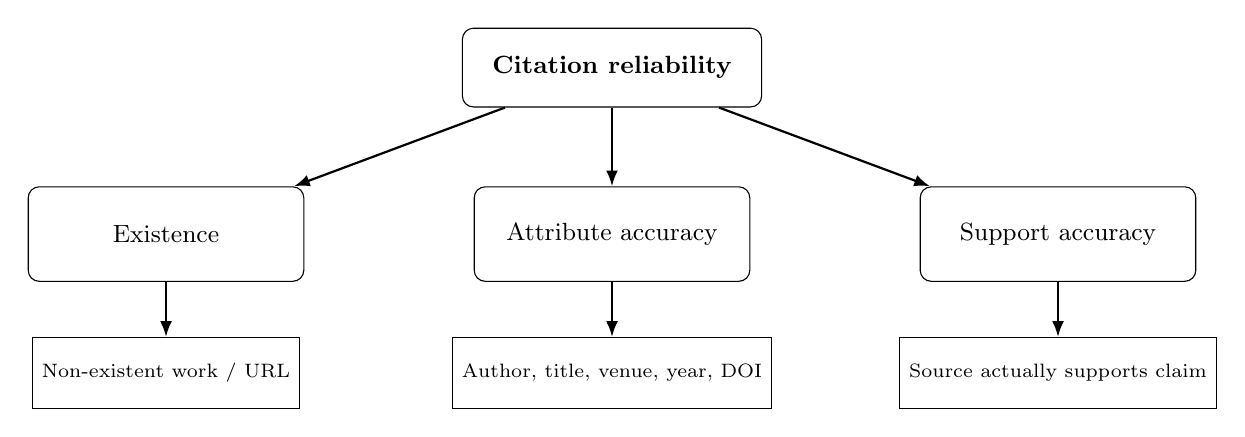
\begin{tikzpicture}[
  root/.style={draw, rounded corners, align=center, minimum width=38mm, minimum height=10mm, font=\small\bfseries},
  cat/.style={draw, rounded corners, align=center, minimum width=35mm, minimum height=12mm, font=\small},
  leaf/.style={draw, align=center, minimum width=30mm, minimum height=9mm, font=\scriptsize},
  arrow/.style={-{Latex[length=2mm]}, thick}
]
\node[root] (root) {Citation reliability};
\node[cat, below left=10mm and 20mm of root] (exist) {Existence};
\node[cat, below=10mm of root] (attr) {Attribute accuracy};
\node[cat, below right=10mm and 20mm of root] (support) {Support accuracy};
\node[leaf, below=7mm of exist] (fake) {Non-existent work / URL};
\node[leaf, below=7mm of attr] (meta) {Author, title, venue, year, DOI};
\node[leaf, below=7mm of support] (claim) {Source actually supports claim};
\draw[arrow] (root) -- (exist);
\draw[arrow] (root) -- (attr);
\draw[arrow] (root) -- (support);
\draw[arrow] (exist) -- (fake);
\draw[arrow] (attr) -- (meta);
\draw[arrow] (support) -- (claim);
\end{tikzpicture}%
}
\caption{Taxonomy used in this review to separate citation existence, bibliographic attribute accuracy, and claim-support accuracy.}
\Description{Taxonomy diagram with citation reliability divided into existence, attribute accuracy, and support accuracy, with examples under each category.}
\label{fig:taxonomy}
\end{figure*}

\subsection{Comparative rates by system class}
Table~\ref{tab:rates} summarizes representative, independently reported fabrication or hallucination rates drawn from the studies reviewed above, organized by system class. Rates are not directly comparable across rows because sample sizes, domains, prompting strategies, and verification methodologies differ substantially (see Section~\ref{sec:challenges}); the table should be read as an ordinal summary of where the empirical literature currently locates each class of system, not as a precision leaderboard.

\begin{table*}[t]
\centering
\caption{Representative citation fabrication / hallucination rates by system class}
\label{tab:rates}
\scriptsize
\begin{tabularx}{\textwidth}{P{2.05cm} P{2.55cm} P{3.0cm} P{2.35cm} Y}
\toprule
\textbf{System class} & \textbf{Representative system(s)} & \textbf{Reported rate} & \textbf{Domain / dataset} & \textbf{Source}\\
\midrule
Unaugmented chat LLM (earlier generation) & ChatGPT-3.5 & 55\% fully fabricated citations & Multidisciplinary literature reviews & Walters \& Wilder (2023)\\
Unaugmented chat LLM (later generation) & ChatGPT-4 & 18\% fully fabricated citations & Multidisciplinary literature reviews & Walters \& Wilder (2023)\\
Unaugmented chat LLM & ChatGPT-3.5 & 47\% fabricated / 46\% authentic-but-inaccurate / 7\% accurate & Medical short papers & Bhattacharyya et al. (2023)\\
Unaugmented chat LLM & ChatGPT-3.5 & 64\% fabricated & Radiology Q\&A & Wagner \& Ertl-Wagner (2024)\\
Unaugmented chat LLM & ChatGPT-3.5 / Bard & 6\% / 0\% citation accuracy & Psychiatry literature search & McGowan et al. (2023)\\
Unaugmented chat LLM (multi-model, systematic review replication) & GPT-3.5, GPT-4, Bard & 28--91\% hallucinated references; precision $\leq$13.4\% & Shoulder/rotator-cuff systematic reviews & Chelli et al. (2024)\\
Meta-analytic synthesis (6 studies) & Mixed chat LLMs & 51\% aggregate (range 47--69\%) & Multidisciplinary & Walters \& Wilder (2023), citing prior work\\
Legal-domain unaugmented LLM & GPT-4 and other public LLMs & $\geq$58\% hallucination on legal queries & U.S. case law & Dahl et al. (2024)\\
Generative / RAG search engine & Bing Chat, NeevaAI, Perplexity.ai, YouChat & 51.5\% of statements fully cite-supported; 74.5\% citation precision & Open web queries & Liu et al. (2023)\\
Citation-generation benchmark (best systems) & Multiple LLM + retriever pipelines & $\sim$50\% lack complete citation support & ELIS (ALCE benchmark) & Gao et al. (2023)\\
Commercial RAG legal-research tool & Lexis+ AI, Westlaw AI-Assisted Research, Casetext CoCounsel & 17--33\% hallucinated or incomplete & U.S. legal research queries & Magesh et al. (2025)\\
Deep research agent (citation accuracy) & Perplexity Deep Research & 90.24\% citation accuracy (highest of tested agents) & DeepResearch Bench (100 PhD-level tasks) & Du et al. (2025)\\
Deep research agents vs. search-augmented LLMs (URL-level) & 10 commercial models/agents & 3--13\% hallucinated URLs; 5--18\% non-resolving overall; agents hallucinate URLs at higher rates than search-augmented LLMs despite denser citation & DRBench (53,090 URLs) \& ExpertQA (168,021 URLs) & Rao et al. (2026)\\
\bottomrule
\end{tabularx}
\end{table*}

\subsection{Interpreting the pattern}\label{sec:pattern}
Three patterns emerge from Table~\ref{tab:rates}. First, within a single vendor's model lineage, capability improvements substantially reduce --- but do not eliminate --- fabrication: GPT-4's fabrication rate is roughly one-third of GPT-3.5's on comparable tasks \citep{walters2023}. Second, retrieval augmentation reliably reduces fabrication relative to unaugmented generation, but the reduction is partial rather than categorical. Commercial legal RAG tools cut hallucination roughly in half or more relative to bare LLMs on similar legal tasks \citep{magesh2025,dahl2024}, and the best deep-research agents reach citation accuracy above 90\% on curated benchmark tasks \citep{du2025} --- yet independent, adversarially designed audits using an external ground-truth source (the Wayback Machine) still find measurable hallucination rates of 3--13\% even in these more sophisticated systems \citep{rao2026}. Third, and most consequential for the framing of this paper, agentic and RAG-based systems introduce a qualitatively distinct risk profile rather than simply a lower version of the chat-model problem: because they issue many more search queries and generate substantially more citations per output than a single chat turn, even a lower per-citation hallucination rate can translate into a comparable or larger absolute number of fabricated citations per report \citep{rao2026}. This ``volume effect'' is a critical, underexplored variable in benchmarking agentic search tools and helps explain why vendor marketing claims of being ``hallucination-free'' (quoted critically in Magesh et al., 2025) have not been borne out by independent audit.

\subsection{Domain sensitivity}\label{sec:domain}
Fabrication and hallucination rates are not domain-invariant. \citet{walters2023} found higher rates in geography than medicine; \citet{rao2026} found non-resolving citation rates ranging from 5.4\% in Business queries to 11.4\% in Theology queries for the same set of systems; and \citet{chelli2024} found substantial variance by systematic-review topic within a single medical subspecialty. This suggests that domain coverage in a model's or agent's underlying training and retrieval corpus, rather than any single architectural property, is a major driver of fabrication risk, and that single-domain benchmarks (e.g., legal-only or medical-only audits) should not be extrapolated to general claims about a system's citation reliability.

\section{Current Approaches and Developments in Detection and Mitigation}\label{sec:mitigation}
\subsection{Self-verification and internal-state probing}
\citet{agrawal2023} proposed treating hallucinated book and article references as a tractable ``model organism'' for studying hallucination more broadly, showing that a model can often be prompted to reveal its own hallucinated references --- without consulting any external resource --- by asking a structured series of direct and indirect follow-up questions about the purported reference's content and authorship; their method achieved high identification accuracy across human expert evaluations. This line of work suggests that some fabricated references are accompanied by internally inconsistent ``knowledge,'' making self-consistency a partially effective, cheap first-pass filter.

\subsection{Sampling-based and retrieval-grounded detection}
\citet{manakul2023} introduced SelfCheckGPT, a zero-resource, black-box method that detects likely-hallucinated content by sampling multiple stochastic generations for the same prompt and measuring their mutual consistency, on the premise that fabricated details vary more across samples than grounded ones. \citet{min2023} introduced FActScore, which decomposes long-form generations into atomic factual claims and verifies each against a trusted knowledge source, reporting that ChatGPT achieved only 58\% factual precision on biography generation and using the metric to compare instruction-tuned, chat-tuned, and retrieval-augmented (PerplexityAI) systems directly. \citet{gao2023} built citation quality directly into the ALCE benchmark's automatic metrics (fluency, correctness, and citation quality), enabling reproducible comparison of citation-grounded generation systems without commercial search-engine dependencies.

\subsection{Reference-specific verification pipelines}
A more recent generation of tools targets bibliographic citations specifically rather than general factual claims. \citet{hu2024} introduced RefChecker, which decomposes model outputs into ``claim-triplets'' checked against a reference under three settings (zero, noisy, and accurate context), outperforming prior fine-grained hallucination checkers by 6.8 to 26.1 points on a curated 11,000-triplet benchmark. \citet{aljamaan2024} developed a ``Reference Hallucination Score'' usability instrument for comparing medical chatbots and search tools (ChatGPT, Bing, SciSpace, Elicit, Bard) across multiple bibliographic-item dimensions, finding ChatGPT-3.5 scored worst overall while Bard failed to generate references at all for the tested prompts --- underscoring that ``no citation'' and ``wrong citation'' are distinct failure modes requiring different scoring treatment. At the level of the published scholarly record, \citet{russinovich2026b} built an automated pipeline that cross-references bibliography entries against arXiv, Semantic Scholar, OpenAlex, CrossRef, DBLP, and the ACL Anthology, escalating unresolved cases to LLM-driven web search before final adjudication --- demonstrating that conference-scale citation auditing is computationally cheap (on the order of cents per paper) even though it remains absent from standard peer-review workflows.

\subsection{URL-level and existence-based verification for agentic systems}
Because agentic search and deep-research tools cite live web URLs rather than only static bibliographic records, verification requires an independent historical ground truth. \citet{rao2026} used the Internet Archive's Wayback Machine to distinguish URLs that never existed (true fabrication) from URLs that existed but later decayed (link rot), a distinction essential for fairly evaluating agentic systems, since both failure modes present identically as ``non-resolving'' at query time. Their study also evaluated post-hoc URL verification and correction as a mitigation layer that can be applied after generation, independent of the underlying model or agent architecture.

\subsection{Retrieval augmentation and citation-constrained generation as first-line mitigations}
Across domains, the single most consistent mitigation strategy in the literature is grounding generation in retrieved source documents at inference time, whether through classical RAG architectures, commercial ``AI-assisted research'' products \citep{magesh2025}, or agentic multi-step search \citep{du2025,rao2026}. The evidence reviewed in Section~\ref{sec:taxonomy} shows this approach reliably reduces --- typically by half or more --- fabrication rates relative to unaugmented generation, even though it does not eliminate the problem, and its residual failure modes (misattributed support, URL hallucination, volume effects) require the detection layers discussed above as a complementary safeguard rather than a substitute.

\begin{table}[t]
\centering
\caption{Comparison of major citation-reliability mitigation approaches.}
\label{tab:mitigation}
\small
\begin{tabularx}{\linewidth}{P{2.4cm} P{3.0cm} Y Y}
\\toprule
\textbf{Approach} & \textbf{Primary target} & \textbf{Strength} & \textbf{Remaining limitation}\\\\
\\midrule
Self-consistency checks & Internal reference inconsistency & Low-cost and model-agnostic first pass & Does not establish that a source exists externally\\\\
Retrieval grounding & Source existence and attribution & Supplies evidence at generation time & Retrieval errors can propagate into the answer\\\\
Citation-quality benchmarks & Claim--source support & Enables reproducible comparison & Benchmark-specific and costly to maintain\\\\
Bibliographic verification & Reference identity and metadata & Directly checks scholarly records & Edge cases include preprints, variants, and incomplete metadata\\\\
Historical URL verification & Web citation existence vs. link rot & Separates fabrication from ordinary URL decay & Requires archive coverage and external access\\\\
Post-hoc correction & User-facing citation reliability & Can be layered onto existing systems & Adds latency and may introduce correction errors\\\\
\\bottomrule
\end{tabularx}
\end{table}

\section{Research Challenges and Limitations}\label{sec:challenges}
\subsection{Inconsistent definitions and non-comparable methodologies}\label{sec:definitions}
The wide range of reported rates in Table~\ref{tab:rates} (roughly 6\% to 91\%) partly reflects genuine differences across systems and time, but is also substantially an artifact of inconsistent operational definitions. Some studies count any bibliographic error as ``hallucination'' (Walters \& Wilder, 2023 treat fabrication and error as separate but related categories), while others restrict the term to identity-level failures and explicitly exclude ordinary bibliographic drift \citep{russinovich2026b}. Verification methods range from manual database lookup \citep{bhattacharyya2023} to automated multi-database cross-referencing with LLM-assisted escalation \citep{russinovich2026b} to independent historical web-archive checks \citep{rao2026}, each with different sensitivity to edge cases such as paywalled, recently published, or non-English sources. This heterogeneity makes direct, apples-to-apples ranking of systems across studies unreliable, and is a central limitation of any synthesis, including this one.

\subsection{Opacity of proprietary agentic systems}
Commercial deep-research agents and RAG-based professional tools are closed systems: their retrieval corpora, ranking and reranking logic, and citation-insertion mechanisms are not publicly documented. \citet{magesh2025} explicitly note that this opacity makes it difficult to attribute observed hallucinations to a specific pipeline stage (retrieval failure, synthesis failure, or citation-insertion failure), and that vendors' own ``hallucination-free'' claims cannot be independently verified without the kind of adversarial, black-box auditing their study undertook. Because vendors also update these systems frequently and without public changelogs, a benchmark result is a snapshot that may not generalize even a few months later.

\subsection{Benchmark and prompt sensitivity}
Reported rates are sensitive to prompt phrasing, requested output length, and task framing. \citet{walters2023} note that ChatGPT rarely produced the requested word count despite explicit instructions, and fabrication rates in several studies varied significantly across prompt variations even within the same system and topic \citep{bhattacharyya2023}. This raises construct-validity concerns for any single-prompt benchmark and argues for multi-prompt, multi-trial designs --- which substantially raise the cost of rigorous evaluation.

\subsection{The moving-target problem}
Because both underlying LLMs and the agentic products built on them are updated on short cycles, benchmarking is chasing a moving target. The comparative advantage documented for GPT-4 over GPT-3.5 \citep{walters2023} or for one deep-research agent over another at a single point in time \citep{du2025} may not hold for subsequent model versions, and no long-lived, continuously updated benchmark yet exists that tracks fabrication rates across model releases at the scale achieved by general capability leaderboards.

\subsection{The volume effect and denominator problems}\label{sec:volume}
As discussed in Section~\ref{sec:pattern}, agentic systems that generate more citations per response complicate simple percentage-based comparisons: a system with a lower per-citation hallucination rate may still expose users to more absolute fabricated citations per report than a system with a higher rate but sparser citation \citep{rao2026}. Few studies report both the rate and the absolute count, and fewer still report user-facing exposure metrics (e.g., expected fabricated citations per session) that would be more directly relevant to real-world risk assessment.

\subsection{Downstream contamination and feedback loops}
Because fabricated citations are entering the peer-reviewed literature \citep{russinovich2026b,sakai2026,ansari2026} and Zhao et al. (2026) show that hallucinated references disproportionately credit already-prominent authors, there is a plausible risk that future LLMs trained on a literature increasingly contaminated by earlier LLM-generated hallucinations will reinforce or compound the problem --- a feedback-loop concern that current benchmarking, which largely treats the training corpus as a fixed and clean reference point, does not yet directly measure.

\section{Research Gaps and Future Directions}\label{sec:gaps}
Building on the challenges above, several concrete directions would materially strengthen the field:

\begin{itemize}
\item \textbf{Standardized, shared definitions and taxonomies.} The field would benefit from converging on the kind of identity-level, drift-excluding definition proposed by \citet{russinovich2026b}, paired with the citation-support/citation-precision distinction from \citet{liu2023} and \citet{gao2023}, so that future studies report comparable, decomposed metrics (existence, attribute accuracy, support accuracy) rather than a single conflated ``hallucination rate.''
\item \textbf{Continuously updated, cross-vendor benchmarks for agentic search.} Existing agentic benchmarks such as DeepResearch Bench \citep{du2025} and the URL-verification methodology of \citet{rao2026} provide strong foundations; extending them into a continuously refreshed, versioned leaderboard --- analogous to general capability leaderboards --- would let practitioners and researchers track whether vendor claims of improvement are empirically substantiated over time, and would help disentangle genuine reliability gains from one-off benchmark overfitting.
\item \textbf{Independent, external ground truth for web-citing systems.} The Wayback Machine approach of \citet{rao2026} should be extended and standardized, since it is currently the only demonstrated method for cleanly separating fabrication from ordinary link rot --- a distinction essential for fair agentic-system evaluation but absent from most existing audits.
\item \textbf{Volume-aware and exposure-based metrics.} Future benchmarks should report absolute fabricated-citation counts and user-facing exposure estimates alongside percentage rates, particularly for agentic systems whose citation density varies widely, to better reflect real-world risk (Section~\ref{sec:volume}).
\item \textbf{Cross-lingual and cross-domain coverage.} Most reviewed studies concentrate on English-language, Western academic or legal sources; \citet{mcgowan2023} is a partial exception in testing Spanish and Italian queries. Given the domain sensitivity documented in Section~\ref{sec:domain}, systematic multilingual and multi-jurisdictional benchmarking is a clear gap, especially as agentic tools are deployed globally.
\item \textbf{Feedback-loop and corpus-contamination studies.} Longitudinal research is needed to test whether training corpora increasingly populated with LLM-fabricated citations \citep{zhao2026} measurably degrade the citation reliability of subsequently trained models --- a question current benchmarks, which evaluate models against a nominally clean ground truth, do not directly address.
\item \textbf{Integration of automated verification into peer review and publishing infrastructure.} Given that conference-scale citation auditing has been shown to be inexpensive (on the order of cents per paper; \citet{russinovich2026b}), an important applied research direction is the integration of tools such as RefChecker \citep{hu2024} directly into submission and review systems, alongside empirical study of their false-positive/false-negative trade-offs at scale and their effect on reviewer workload and author burden.
\item \textbf{Transparency requirements or standardized audit protocols for commercial agentic tools.} Given the opacity problem documented in Section~\ref{sec:challenges}, the field would benefit from either vendor-supported evaluation APIs or agreed-upon third-party audit protocols --- modeled on the adversarial methodology of \citet{magesh2025} and \citet{rao2026} --- that permit reproducible, independent benchmarking of proprietary systems without requiring vendor cooperation.
\end{itemize}

\section{Synthesis of Evidence}\label{sec:synthesis}
Taken together, the literature supports a layered interpretation rather than a single universal ``hallucination rate.'' Unaugmented generation can produce high rates of fabricated or inaccurate references in some domains, while retrieval and agentic search reduce some failure modes but introduce additional evaluation questions around citation support, URL validity, and citation volume. The strongest studies therefore evaluate multiple properties separately. Figure~\ref{fig:taxonomy} captures this distinction, while Table~\ref{tab:mitigation} shows why no single mitigation addresses every layer.

Three conclusions follow from this synthesis. First, reported percentages should always be interpreted together with the system, domain, prompt, denominator, and verification protocol. Second, citation accuracy and citation quantity should be reported together for agentic systems because Equation~\eqref{eq:volume-effect} makes their relationship explicit. Third, reproducible external verification is increasingly important: recent work has demonstrated that large-scale auditing of both scholarly references and web URLs is technically feasible, making independent verification a realistic complement to model-side safeguards.

\section{Conclusion}\label{sec:conclusion}
Citation fabrication is a well-documented, quantifiable, and still largely unsolved failure mode of large language models and the agentic search tools built on them. The evidence surveyed here shows a consistent, if imperfect, gradient of improvement: unaugmented early chat models fabricate references at rates often exceeding 30\%; later-generation models and retrieval-augmented professional tools roughly halve that rate; and the most capable agentic deep-research systems can achieve citation accuracy above 90\% on curated benchmarks, yet still exhibit measurable --- and in some respects distinctive --- fabrication when audited against independent, adversarial ground truth, in part because their higher citation volume can offset lower per-citation error rates. The consequences are no longer confined to individual user interactions: fabricated citations have been documented inside the peer-reviewed literature at flagship AI conferences and across the broader scholarly corpus, raising the prospect of a slow, self-reinforcing contamination of the record that future models may in turn be trained on. Meaningful progress will require not only continued architectural and retrieval improvements, but also methodological convergence --- shared definitions, external ground truth, volume-aware metrics, and reproducible cross-vendor auditing --- so that the field can move from a patchwork of individually valuable but hard-to-compare studies toward a genuinely cumulative science of citation reliability.

\bibliographystyle{ACM-Reference-Format}
\bibliography{references}
\end{document}
